\section{The ``Scanning" tangle Drawing Algorithm}

We present a 1-tangle drawing algorithm and a proof of its validity. We call it the ``Scanning" tangle drawing algorithm because one can picture it as a process similar to a braiding board but upside down. The pieces of our finished diagram are attached to the braiding board, and we hold a set containing crossings that we still need to attach. We ``scan" the diagram already on the braiding board and try to find a crossing that we can attach. The scanning must be precise and greedy, otherwise the method is not guaranteed to work. The generic steps of the algorithm can be seen in \Cref{fig:scan}. We now give the algorithm again but more precisely:

% draw each step
\begin{enumerate}
\item Label each segment between the crossings of the tangle. Consider the set of crossings with each end labeled according to the respective connections in the tangle. 
\item Take the first crossing that we encounter along the tangle, leave the end from which we came and attach the three other ends to the scanning front.
\begin{figure}[!h]
\centering
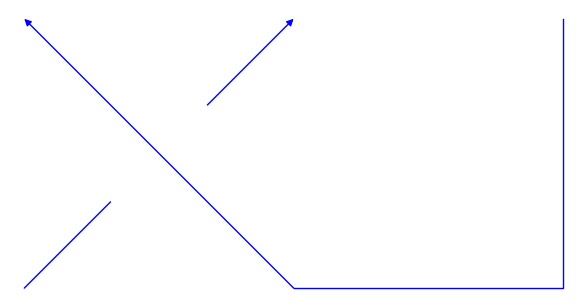
\includegraphics[width=0.4\textwidth]{scanning_0.png}
\caption{The first crossing, the left incoming strand we leave be, the right incoming strand we raise to the ``scanning" front.}
\end{figure}
\item At each iteration read the labels of pairs of ends attached to the front from left to right, and attempt one of the following
\begin{enumerate}
\item If possible attach a new crossing to the two strands, if there exists an unused crossing with those labels (we allow rotating the crossings)
\item If possible attach a new crossing to the left strand, if there exists an unused crossing with that label
\item If neither are possible, try to "cap" off the strands, if they have the same label.
\end{enumerate}
If none of this is possible with the pair, consider the next pair given by the right strand of the previous pair and the strand to the right of it. If none of the consecutive pairs work, then try (b) with the right-most strand.
\begin{figure}[h!]
\centering
\begin{subfigure}[t]{0.3\textwidth}
\centering
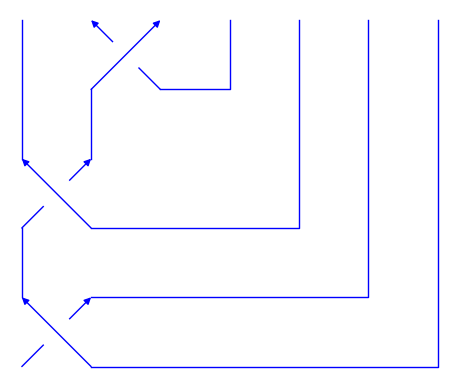
\includegraphics[width=\textwidth]{scanning_2.png}
\caption{Attaching two strands}
\label{fig:scan1}
\end{subfigure}
\hfill
\begin{subfigure}[t]{0.3\textwidth}
\centering
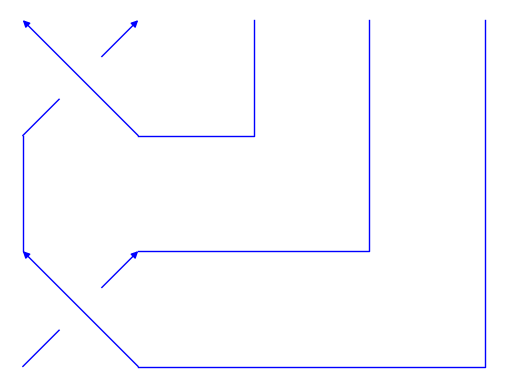
\includegraphics[width=\textwidth]{scanning_1.png}
\caption{Attaching one strand}
\label{fig:scan2}
\end{subfigure}
\hfill
\begin{subfigure}[t]{0.25\textwidth}
\centering
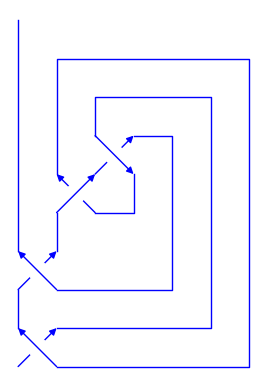
\includegraphics[width=0.8\textwidth]{scanning_3.png}
\caption{Closing a "cap"}
\label{fig:scan3}
\end{subfigure}
\caption{What iterations of the scanning method look like}
\label{fig:scan}
\end{figure}
\item If there is only one strand left on the front, we are done, if there are more, repeat the previous step.
\end{enumerate}

\begin{proof}
What our algorithm essentially does is provide a nice drawing of the tangle diagram, nice in the sense that it aims to not produce extra crossings in the process. It is given that the tangle diagram is planar by definition, so if at every step the diagram with scanning front is planar, then we are guaranteed to have a planar drawing, with no extra crossings.

We see that at the first step, when we fix the first crossing, the diagram is planar. Suppose at some iteration of the algorithm we have a planar diagram, then by affixing a crossing or capping off two strands we do not change the planarity of the diagram. Hence once the algorithm terminates, we have a planar tangle diagram.
\end{proof}


